\chapter{Hierarchy of Stochastic Pure States}
\label{chap:num}
% * numerical treatments necessary
% * main goal: calculate reduced density operator
% * other things: absorption spectra, single trajectories
%

The Jaynes-Cummings model from the last chapter is one of the rare cases where an analytical ansatz for $\bar O$ is known.
Numerical solution-methods of the convolutionless non-Markovian stochastic Schrödinger equation usually attack the consistency condition~\ref{eq:nmqsd.consistency_condition} directly using an expansion of $\bar O$ with respect to the noise \cite{YuDiGiSt99_pertubation,RiRoSt11_fmo}.
Although this provides an efficient algorithm for large parameter regimes, the problems presented in the last chapter impede systematic improvements.

With recent advances in super-computing, realistic biological and chemical systems came within the reach of the far more costly, but better-behaved and formally exact hierarchical-equations-of-motion (\HEOM) approach \cite{Ta06_stochastic}.
Although formally equivalent to the Feynman-Vernon influence functional, the \HEOM-formalism is much better suited for numerical investigations, since it provides a systematic way to check convergence and does not require evaluation of highly-oscillatory path integrals.
Summarized shortly, it amounts to dealing with memory effects in the influence-functional by introducing additional auxiliary density matrices (ADMs).
Therefore, the single equation of motion for $\rho_t$ is transfered into a much simpler hierarchy of memory-less differential equations, which allows for a straightforward numerical integration.
However, the number of ADMs grows rapidly for highly non-Markovian systems.
Combined with the $N^2$-scaling of the memory requirement\footnote{%
  Sparse.matrix algorithms are able to reduce the $N^4$-scaling of the propagation matrices, but still, these are even more problematic than the ADMs.
}
with the system's dimension $N$, this places enormous demands on the computational infrastructure.\\



It this chapter, we present the main result of this work: a hierarchy of stochastic, pure state trajectories in the spirit of the established \HEOM-formalism.
At the beginning, we derive the pure-state hierarchy based on the \NMSSE in its linear, as well as nonlinear version.
%As  closed set of equations crucially relies on an exponential bath correlation function (or sums thereof), \autoref{sec:num.expansion} is devoted to an expansion of more general spectral densities at finite temperature leading to the sought-after form.
Since the derivation of the hierarchy crucially relies on an exponential bath-correlation function (or sums thereof), \autoref{sec:num.expansion} is devoted to an expansion of more general spectral densities at finite temperature providing the necessary form.
Finally, we apply the hierarchy of stochastic pure states to the Spin-Boson model, investigating its accuracy in dependence on the sample size and number of auxiliary states.


%%%%%%%%%%%%%%%%%%%%%%%%%%%%%%%%%%%%%%%%%%%%%%%%%%%%%%%%%%%%%%%%%%%%%%%%%%%%%%%
\section{Derivation of the Hierarchy}
\label{sec:num.sheom}
% * main idea
%
%%%%%%%%%%%%%%%%%%%%%%%%%%%%%%%%%%%%%%%%%%%%%%%%%%%%%%%%%%%%%%%%%%%%%%%%%%%%%%%

In this section, we present the main results of this work, namely an approach to solve the non-Markovian stochastic Schrödinger equation
\begin{equation}
  \partial_t \psitZ = -\ii h \psitZ + L\ZZ_t \psitZ - \adj{L}\int_0^t \alpha(t-s) \frac{\delta\psitZ}{\delta\ZZ_s} \dd s
  \label{eq:num.nmsse}
\end{equation}
numerically without resorting to the $O$-operator substitution.
Therefore, we need to conceive a different way to deal with the non-locality of the functional derivative with respect to time and process realization, as it prevents the application of efficient Monte-Carlo methods, which are used to deal with stochastic Schrödinger equations in the Markovian regime \cite{Ca93_quantum_optics,Pe98_qsd}.
It turns out that for certain correlation functions the linear \NMSSE~\ref{eq:num.nmsse} is formally equivalent to an infinite hierarchy of completely local stochastic differential equations.

%%%%%%%%%%%%%%%%%%%%%%%%%%%%%%%%%%%%%%%%%%%%%%%%%%%%%%%%%%%%%%%%%%%%%%%%%%%%%%%
\subsection{Linear Hierarchy}
\label{sub:num.sheom.lin}
% * derivation
% * terminator
%

The basic idea is to absorb the action of the functional derivative on $\psitZ$ into an auxiliary pure state
\begin{equation}
  \psitZ[1] := \int_0^t \alpha(t - s) \frac{\delta \psi_t(\ZZ)}{\delta \ZZ_s} \dd s.
  \label{eq:num.first_order}
\end{equation}
Hereinafter, we use the term \quotes{state} quite loosely for any vector in the system's Hilbert space regardless of its norm.
Recall that the integral boundaries arise only after we apply the derivative on states $\psi_t(\ZZ)$ that satisfy the additional condition $\delta \psitZ / \delta \ZZ_s = 0$ for $ s < 0$ and $s > t$.
Therefore, we may write \autoref{eq:num.first_order} more concisely as
\begin{equation*}
  \psitZ[1] = \left( \int \alpha(t - s) \frac{\delta}{\delta \ZZ_s} \dd s \right) \psitZ =: \adjZZ_t \psitZ
\end{equation*}
with the integrated functional derivation operator $\adjZZ_t$.
For a finite environment, $\adjZZ_t$ is simply the representation of the force operator~\ref{eq:nmqsd.force_operator} in the time-independent coherent state basis.

The equation of motion for $\psitZ[1]$ takes a form similar to the original \NMSSE~\ref{eq:num.nmsse}, provided $\dot\adjZZ_t = \int\dot\alpha(t-s) \, \delta / \delta \ZZ_s \dd s$ can be expressed in terms of known quantities.
Of course, the simplest choice is an exponential bath correlation function
\begin{equation}
  \alpha(t) = g \, \exp[-\gamma \abs{t} - \ii \Omega t]
  \label{eq:num.exp_bcf}
\end{equation}
with $g$, $\gamma$ and $\Omega$ real.
The absolute value of $t$ in the exponent is necessary to ensure hermiticity $\alpha(-t) = \cc{\alpha(t)}$.
In \autoref{sec:hierarchy.memory_integral} we elaborate that such a correlation function simply gives
\begin{equation}
  \dot\adjZZ_t \psitZ = - (\gamma + \ii \Omega) \adjZZ_t\psitZ
  \label{eq:num.dot_adjZZt}
\end{equation}
for solutions $\psitZ$ of the \NMSSE with vacuum initial conditions.
We abbreviate the coefficient $w = \gamma + \ii\Omega$ in order to simplify notation.\\



Now, let use return to the {\NMSSE}.
With the auxiliary stochastic state~\ref{eq:num.first_order} it can be expressed as an inhomogeneous stochastic equation, namely
\begin{equation*}
  \partial_t \psitZ = -\ii\Hsys\psitZ + L\ZZ_t\psitZ - \adj{L}\psitZ[1].
\end{equation*}
By the construction in the previous paragraph, the last term satisfies the closely related equation
\begin{align}
  \partial_t (\adjZZ_t \psi_t) &= - w \adjZZ_t\psi_t + \adjZZ_t ( -\ii\Hsys + L\ZZ_t - \adj{L} \adjZZ_t ) \psi_t \nonumber \\
  &= (-\ii\Hsys - w + L\ZZ_t) \psit[1] + [\adjZZ_t, \ZZ_t] L\psit - \adj{L} \adjZZ_t \psit[1].
  \label{eq:num.dot_psi1}
\end{align}
Naturally, $\adjZZ_t$ commutes with all system operators and itself.
Not surprising, the functional derivative reappears in the equation for $\psit[1]$, therefore, we need to introduce another auxiliary state $\psitZ[2]$.
This scheme leads to an infinite hierarchy of stochastic vectors in the system's Hilbert space
\begin{equation}
  \psitZ[k] := \adjZZ_t \psitZ[k-1] = \adjZZ_t^k \psitZ.
  \label{eq:num.auxiliary_states}
\end{equation}
Expressed in the new auxiliary states and with $[\adjZZ_t, \ZZ_s] = \alpha(t-s)$, \autoref{eq:num.dot_psi1} reads
\begin{equation*}
  \partial_t \psitZ[1] = (-\ii\Hsys - w + L\ZZ_t) \psitZ[1] + \alpha(0) L\psitZ[0] - \adj{L}\psitZ[2].
\end{equation*}
Along these lines it is straightforward to derive the full hierarchy of equations of motions for all $\psit[k]$.
Since the commutator $[\adjZZ_t, \ZZ_s]$ is a $\Complex$-number, each auxiliary state only couples to the order directly above and below
\begin{equation}
  \partial_t\psitZ[k] = (-\ii\Hsys - kw + L\ZZ_t)\psitZ[k] + k \alpha(0) \psitZ[k-1] - \adj{L} \psitZ[k+1].
  \label{eq:num.hierarchy_lin}
\end{equation}
The vacuum initial condition for the true quantum trajectory $\delta \psi_0 / \delta \ZZ_s = 0$ requires all auxiliary states to vanish at $t=0$.

Of course the infinite hierarchy is even more intricate to solve than the original {\NMSSE}.
To transform \autoref{eq:num.hierarchy_lin} into a practical scheme, we truncate the hierarchy at finite order.
It is quite remarkable that this can be done in a self-consistent manner, which even incorporates the neglected orders approximately.
This is derived most clearly using the equivalent integral equation for $\psit[k]$ (with $w = \gamma + \ii\Omega$ reinserted)
\begin{align}
  \psitZ[k] = \int_0^t &\exp[-k\gamma(t-s) - \ii k\Omega(t-s)] \times \nonumber\\
  &\times \Texp[\int_s^t -\ii\Hsys + L\ZZ_u \dd u] \left( k \alpha(0)L\psi_s^{(k-1)}(\ZZ) - \adj{L} \psi_s^{(k+1)}(\ZZ) \right) \dd s,
  \label{eq:num.terminator_integral}
\end{align}
as it satisfies \autoref{eq:num.hierarchy_lin} and the correct initial conditions.
Here, $T_+$ denotes positive time-ordering.
Under the condition $k\gamma \gg \omega_\mathrm{sys}$, where $\omega_\mathrm{sys}$ is a typical frequency for the system's free time evolution, the first exponential drops to zero before the remaining integrand changes noticeably.
Therefore, the latter can be safely extracted from the integral setting $s \approx t$
\begin{equation*}
  \psitZ[k] = \left( k \alpha(0)L\psitZ[k-1] - \adj{L} \psitZ[k+1] \right) \int_0^t \exp[-kw(t-s)]  \dd s,
\end{equation*}
Evaluating the rest of the integral simply gives $\frac{1 - \exp(-kwt)}{kw}$.
As the second summand is relevant only for very small times $t$, it is dropped in the following work---including it in a numerical implementation does not pose any additional difficulties.
Thus, we have an approximate expression for the $k$\th-order auxiliary state
\begin{equation}
  \psitZ[k] = \frac{\alpha(0)}{w} L\psitZ[k-1] - \frac{1}{kw} \adj{L} \psitZ[k+1].
  \label{eq:num.almost_terminator}
\end{equation}
If we further assume that the second term, coupling to the order above, is suppressed by the prefactor $\frac{1}{kw}$, the infinite hierarchy terminates at finite order.
However, since there is no simple assessment for the order of magnitude of individual auxiliary states $\psitZ[k]$, this assumption needs to checked for each calculation separately by increasing the truncation order.
The remainder of \autoref{eq:num.almost_terminator}, namely
\begin{equation}
  \psitZ[k] = \frac{\alpha(0)}{w} L \psitZ[k-1],
  \label{eq:num.terminator}
\end{equation}
is called \quotes{\emph{terminator}} of the hierarchy.
This procedure can be interpreted as a Markov approximation for the $(k-1)$\th auxiliary state similar to \autoref{eq:nmqsd.markov}, since the memory-integral is replaced by a time-local expression.

Remarkably, the above argument does not solely rest on the exponential suppression by $\exp[-k\gamma(t-s)]$ in \autoref{eq:num.terminator_integral}.
As the results from \autoref{sec:app.spectra} show, the hierarchy even terminates for $\gamma = 0$ due to the highly oscillatory $\exp[-\ii k \Omega(t-s)]$.
Therefore, we propose a truncation criterion related to the one used within the \HEOM-formalism \cite{Ta06_stochastic}
\begin{equation}
  k(\gamma + \abs{\Omega}) \gg \omega_\mathrm{sys},
  \label{eq:num.truncation_condtion}
\end{equation}
which we will test in \autoref{sub:num.spin_boson.depth}.
It turns out that \autoref{eq:num.truncation_condtion} is not a good criterion, since it neglects the crucial influence of the coupling strength $g$.
So once again, in practical applications it is much more conclusive to check convergence of the results with the truncation order for each set of parameters individually.

%%%%%%%%%%%%%%%%%%%%%%%%%%%%%%%%%%%%%%%%%%%%%%%%%%%%%%%%%%%%%%%%%%%%%%%%%%%%%%%
\subsection{Nonlinear Hierarchy}
\label{sub:num.sheom.nonlin}
% * derivation

We mentioned in \autoref{sec:nmqsd.nonlin_nmsse} how the efficiency of the Monte-Carlo scheme improves greatly, if we use comoving environmental basis states~\ref{eq:nmqsd.comoving_flow} and the corresponding nonlinear {\NMSSE}.
Up to a certain extend this idea can also be applied to our hierarchical equations of motion.

Seen as a function of coherent state labels $\cc\zz$ instead of the process $\ZZ$, the Girsanov-transformed auxiliary states are defined by
\begin{equation*}
  \tilde\psi_t^{(k)}(\cc\zz) := (\psit[k] \circ \vec\phi_t)(\cc\zz) = \psit[k](\vec\phi_t(\cc\zz))
\end{equation*}
with the \quotes{phase-space} flow~\ref{eq:nmqsd.comoving_flow}.
Then, along the lines of the derivation leading to \autoref{eq:num.hierarchy_lin} we obtain its nonlinear form
\begin{align}
  \partial_t \tilde\psi_t^{(k)}(\cc\zz) &= \left( -\ii\Hsys - kw + L\ZZ_t + L \int_0^t \cc{\alpha(t-s)} \qmean{\adj L}_s \dd s \right)\tilde\psi_t^{(k)}(\cc\zz) \nonumber\\
  &+ k \alpha(0) L \tilde\psi_t^{(k-1)} - (\adj{L} - \qmean{\adj L}_t) \tilde\psi_t^{(k+1)}(\cc\zz),
  \label{eq:num.hierarchy_nonlin}
\end{align}
with the normalized expectation value taken with respect to the true quantum trajectory---or, put differently, with respect to the zeroth order auxiliary state
\begin{equation}
  \qmean{\adj L}_t = \frac{\bra{\tilde\psi_t^{(0)}(\ZZ)} \adj{L} \ket{\tilde\psi_t^{(0)}(\ZZ)}}{\braket{\tilde\psi_t^{(0)}(\ZZ)}{\tilde\psi_t^{(0)}(\ZZ)}}.
  \label{eq:num.qmean}
\end{equation}
Deriving a terminator for the nonlinear version is completely analog to \autoref{eq:num.terminator} and gives the same result.

Notice that the exponential correlation function necessary for the hierarchy also simplifies the treatment of the memory-term in \autoref{eq:num.hierarchy_nonlin}.
Indeed $f(t) := \int_0^t \cc{\alpha(t-s)} \qmean{\adj L}_s \dd s$ satisfies
\begin{equation}
  \dot f(t) = \alpha(0) \qmean{\adj L}_t - \cc{w} f(t).
  \label{eq:num.memory_term}
\end{equation}
Therefore, we only need to store the hierarchy and auxiliary function $f$ for one time step in a numerical implementation---making this approach very memory-efficient.

But one caveat remains: For the convolutionless formulation we can go one step further and derive an equation for normalized pure state trajectories~\ref{eq:nmqsd.nmsse_nonlin_full}.
However, such a hierarchy with all auxiliary states having unit norm seems to be unobtainable.
Nonetheless, we expect that there is another version of the nonlinear hierarchy, which achieves a normalized zero-order state---this would tremendously improve the numerical accuracy of the expectation values~\ref{eq:num.qmean} for large $\braket{\tilde\psi_t^{(0)}(\ZZ)}{\tilde\psi_t^{(0)}(\ZZ)}$\footnote{%
  I would like to thank Richard Hartmann for pointing this out.
}.



%%%%%%%%%%%%%%%%%%%%%%%%%%%%%%%%%%%%%%%%%%%%%%%%%%%%%%%%%%%%%%%%%%%%%%%%%%%%%%%
\subsection{Multiple Bath-Modes}
\label{sub:num.sheom.nonlin}
% * rectangular vs triangular truncation

Of course, most interesting systems cannot be modeled using a single exponential decaying correlation function~\ref{eq:num.exp_bcf}.
To accommodate a more complex environmental structure, we modify the hierarchy to handle a finite number of exponential modes coupling to the system with arbitrary operators.
As the crucial points do not depend on the choice of linear or nonlinear version, we are only concerned with the former in this section to simplify notation.

The linear \NMSSE for a finite number $N$ of independent environments is derived similarly to the lines of \autoref{sec:nmqsd.lin_nmsse} and reads
\begin{equation}
  \partial_t \psit = -\ii\Hsys\psit + \sum_{j=1}^N L_j \ZZ_{j, t} \psit - \sum_{j=1}^N \adj{L}_j \int_0^t \alpha_j(t - s) \frac{\delta \psit}{\delta \ZZ_{j, t}} \dd s
  \label{eq:num.nmsse_multimode}
\end{equation}
with mutually independent noise processes satisfying
\begin{equation*}
  \E\,Z_{i, t} = 0, \quad \E\,Z_{i, t} Z_{j, s} =0, \quad\mbox{and}\quad \E\,Z_{i, t} \ZZ_{j, s} = \delta_{ij}\alpha_i(t-s).
\end{equation*}
Just as in the single-mode case, \autoref{eq:num.nmsse_multimode} is equivalent to an infinite hierarchy of auxiliary states if all correlation functions take the exponential form~\ref{eq:num.exp_bcf}.
Since all derivation operators $\adjZZ_{j, t}$ corresponding to the processes $\ZZ_{j, t}$ mutually commute, the most general form of an auxiliary state is given by
\begin{equation}
  \psit[k_1, \dots, k_N] := \adjZZ_{1, t}^{k_1} \dots \adjZZ_{N, t}^{k_N} \psit.
  \label{eq:num.auxiliary_states_multi}
\end{equation}
Hereinafter, we use boldface symbols to abbreviate $N$-tuples such as $\kk = (k_1,\dots,k_n)$.
Summarily, the infinite hierarchy appertaining to \autoref{eq:num.nmsse_multimode} reads
\begin{equation}
  \partial_t\psit[\kk] = \left( -\ii\Hsys - \kk\cdot\ww + \sum_j L_j \ZZ_{j, t} \right) \psit[\kk] + \sum_j k_j \alpha_j(0) \psit[\kk - \ee_j] - \sum_j \adj{L}_j \psit[\kk + \ee_j],
  \label{eq:num.hierarchy_lin_multi}
\end{equation}
where $\ee_j$ denotes the $j$-th unit vector in $\Reals^N$ and $\kk\cdot\ww = \sum_j k_jw_j$ is the euclidean scalar product\footnote{%
  Although $\ww$ is complex in general, the scalar product $\kk\cdot\ww$ does not involve complex conjugation.
}.\\

%% Truncation schemes %%%%%%%%%%%%%%%%%%%%%%%%%%%%%%%%%%%%%%%%%%%%%%%%%%%%%%%%%%
%\begin{figure}
%  \centering
%  \begin{subfigure}[b]{.4\columnwidth}
%    \centering
%    \includegraphics[scale=.85]{img/cubic_hierarchy}
%    \caption{Cubic}
%    \label{fig:num.trunc_cubic}
%  \end{subfigure}
%  \begin{subfigure}[b]{.4\columnwidth}
%    \centering
%    \includegraphics[scale=.85]{img/triang_hierarchy}
%    \caption{Triangular}
%    \label{fig:num.trunc_tria}
%  \end{subfigure}
%  \caption{Comparison of the two truncation schemes in the special case of $N=2$ processes with order $D$.}
%  \label{fig:num.trunc}
%\end{figure}
%%%%%%%%%%%%%%%%%%%%%%%%%%%%%%%%%%%%%%%%%%%%%%%%%%%%%%%%%%%%%%%%%%%%%%%%%%%%%%%%

When it comes to truncating the hierarchy~\ref{eq:num.hierarchy_lin_multi} the most obvious strategy is simply to cut off each mode separately at given order $D$.
In other words the truncation condition reads $0 \le k_j \le D$ for all $j=1,\dots,N$; any auxiliary state not satisfying it is either set to zero or replaced by the terminator
\begin{equation*}
  \psi^{(\kk+\ee_j)}
  = \sum_i  \frac{(\kk + \ee_j)_i \, \alpha_i(0)}{(\kk+\ee_j)\cdot\vec{w}} \op{L_i} \psi^{(\kk +\ee_j - \ee_i)}_t.
\end{equation*}
We refer to this as the \quotes{cubic truncation scheme} since the hierarchy's shape resembles an $N$-cube. % as shown for $N=2$ in \autoref{fig:num.trunc_cubic}.
Clearly, the number of auxiliary states scales exponentially like $(D+1)^N$, which makes the treatment of large systems with a highly structured spectral density virtually impossible.

%% Scaling behavior %%%%%%%%%%%%%%%%%%%%%%%%%%%%%%%%%%%%%%%%%%%%%%%%%%%%%%%%%%%%
\begin{figure}
  \centering
  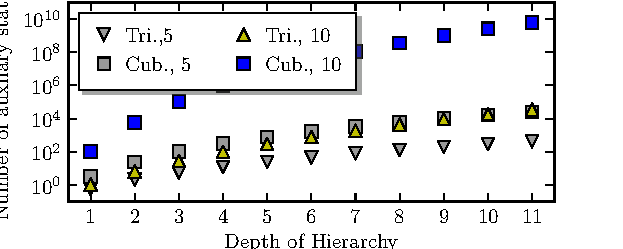
\includegraphics{img/scaling.pdf}
  \caption{%
    Scaling of the number of auxiliary states with the truncation order $D$ and number of modes $N$.
    Even for relatively small $N$, the triangular scheme~\ref{eq:num.triangular_scaling} is far superior compared to the cubic truncation scheme with an exponential scaling law $(D+1)^N$.
  }
  \label{fig:num.scaling}
\end{figure}
%%%%%%%%%%%%%%%%%%%%%%%%%%%%%%%%%%%%%%%%%%%%%%%%%%%%%%%%%%%%%%%%%%%%%%%%%%%%%%%%

Examining \autoref{eq:num.hierarchy_lin_multi} closer, we notice that the term responsible for suppression of the $\kk$\th auxiliary state is $\exp(-\kk \cdot \ww)$.
Instead of treating each mode individually, we use a condition better suited for the product $\kk\cdot\ww$, namely $0 \le \abs{\kk} \le D$ with $\abs{\kk} = \sum_j k_j$.
%For $N=2$ the corresponding states form a triangular shape as shown in \autoref{fig:num.trunc_tria}---hence the name \quotes{triangular truncation scheme}.
For $N=2$ the corresponding states form a triangular shape---hence the name \quotes{triangular truncation scheme}.
The appropriate generalization to an arbitrary number of modes is an $N$-simplex with the number of elements given by
\begin{equation}
  \sum_{d=0}^D {d + N - 1 \choose N - 1} = \frac{(D + N)!}{D!N!},
  \label{eq:num.triangular_scaling}
\end{equation}
showing a much softer scaling with $N$ compared to the cubic scheme.
In \autoref{fig:num.scaling} we display the number of auxiliary states required for a given number of modes and truncation order $D$.
Clearly, the triangular truncation is far superior although for small $N$ both methods are applicable.
The difference is more pronounced for larger $N$.

Depending on the specific problem, additional truncation conditions may reduce the computational expenses without sacrificing accuracy.
Especially environments that mix modes with large memory times and almost-Markovian modes provide many options for optimization.
However, we do not elaborate this point any further and rely on the triangular truncation throughout this work.

%%%%%%%%%%%%%%%%%%%%%%%%%%%%%%%%%%%%%%%%%%%%%%%%%%%%%%%%%%%%%%%%%%%%%%%%%%%%%%%
\section{Bath Correlation Function Expansion}
\label{sec:num.expansion}
% * pade spectrum decomposition
% * also mention other (Matsubara e.g.)
% * uniqueness? Theoretically yes, in practices doesnt matter!
% * Plot for Ohmic spectral density (where do these appear?)
% * Show highly structured density, approximation!
%
%      Cool to use antisymmetric lorentzians

%%%%%%%%%%%%%%%%%%%%%%%%%%%%%%%%%%%%%%%%%%%%%%%%%%%%%%%%%%%%%%%%%%%%%%%%%%%%%%%

The applicability of our hierarchical equations of motion to certain models depends predominantly on the ability to express the relevant bath correlation function
\begin{equation}
  \alpha(t-s) = \int_0^\infty J(\omega) \left( \coth \left( \frac{\beta \omega}{2} \right) \cos \omega(t-s) - \ii\sin \omega(t-s) \right) \mathrm{d}\omega
  \label{eq:num.alpha_thermal}
\end{equation}
as a sum of exponentials like~\ref{eq:num.exp_bcf}.
Such exponentials arise as Fourier transforms of a Lorentzian spectral density
\begin{equation}
  J(\omega) = \frac{1}{\pi} \frac{\gamma}{(\omega - \Omega)^2 + \gamma^2}.
  \label{eq:num.lorentzian}
\end{equation}
Hence they can be obtained from \autoref{eq:num.alpha_thermal} in the zero-temperature limit provided we extend the integral domain to include arbitrary negative frequencies as well.
This unphysical assumption seems to be a good approximation to the exact case without negative frequencies for certain parameters as \autoref{fig:num.lorentzian} shows:
For $\gamma\ll\Omega$ the Lorentzian density $J$ is concentrated on the positive semi-axis and the negative frequency contributions vanish primarily.
However, \autoref{eq:num.lorentzian} is a prime example of a heavy-tailed distribution, having no finite moments except $\int J(\omega) \dd \omega = 1$, so this approximation needs to be handled with care.\\



%% Lorentzians %%%%%%%%%%%%%%%%%%%%%%%%%%%%%%%%%%%%%%%%%%%%%%%%%%%%%%%%%%%%%%%%%
\begin{figure}
  \centering
  \includegraphics{img/lorentzian}
  \caption{%
    Schematic comparison of Lorentzian spectral densities used to obtain exponential bath correlation functions (see \autoref{eq:num.lorentzian} for notation).
    For $\gamma\ll\Omega$ (blue line) the weight is concentrated on the positive semi-axis.
  }
  \label{fig:num.lorentzian}
\end{figure}
%%%%%%%%%%%%%%%%%%%%%%%%%%%%%%%%%%%%%%%%%%%%%%%%%%%%%%%%%%%%%%%%%%%%%%%%%%%%%%%%

A more systematic way to obtain the desired bath correlation function in the case $T > 0$ involves anti-symmetrized spectral densities $\tilde J(\omega) := J(\omega) - J(-\omega)$.
This way, negative frequencies are included without any approximation.
Indeed, since $\tilde J$, $\coth$, and $\sin$ are anti-symmetric and $\cos$ is symmetric with respect to reflection at the origin we have
\begin{equation}
  \int_0^\infty \tilde J(\omega) (\dots) \mathrm{d}\omega = \frac{1}{2}\int_{-\infty}^\infty \tilde J(\omega) (\dots) \mathrm{d}\omega.
  \label{eq:num.correlation_integral}
\end{equation}
Commonly used examples are Drude spectral densities in the \HEOM-formalism or sums of anti-symmetrized Lorentzians, which are well suited to approximate highly-structured environments \cite{MeTa99_non_markovian}.
Although the discussion below works for a much larger class of spectral densities \cite{RiEi13_bcf}, we assume $\tilde J$ to have a finite number of mutually distinct poles lying off the real and imaginary axis.

To calculate the correlation function, we evaluate the integral~\ref{eq:num.correlation_integral} analytically using the residue theorem.
While the poles of the anti-symmetric spectral density $\tilde J$ are assumed to be known, there are different expansion schemes for the hyperbolic cotangent:
Since many established \HEOM-results are based on the Matsubara-spectrum decomposition, it is presented in detail.
Nevertheless, it has been brought forward only recently that the Padé-expansion provides superior approximation scheme, especially for low temperature \cite{HuXuYa10_pade,Hu11_pade}.
We achieve a much more convenient form by treating the real and imaginary part of $\alpha(t) = a(t) + \ii b(t)$ separately, where the former
\begin{equation}
  a(t) = \frac{1}{2} \int_{-\infty}^\infty \tilde J(\omega) \coth \left( \frac{\beta\omega}{2} \right) \cos \omega t \dd\omega
  = \frac{1}{2} \int_{-\infty}^\infty \tilde J(\omega) \coth \left( \frac{\beta\omega}{2} \right) \exp[\ii \omega t] \dd\omega,
  \label{eq:num.alpha_thermal_re}
\end{equation}
includes all thermal effects, while the imaginary part
\begin{equation*}
  b(t) = - \frac{1}{2} \int_{-\infty}^\infty \tilde J(\omega) \sin \omega t \dd \omega
  = \frac{1}{2\ii}\int_{-\infty}^\infty \tilde J(\omega) \, \exp[\ii\omega t] \dd\omega
\end{equation*}
is identical for all temperatures.\\



%%%%%%%%%%%%%%%%%%%%%%%%%%%%%%%%%%%%%%%%%%%%%%%%%%%%%%%%%%%%%%%%%%%%%%%%%%%%%%%%
%\subsection{Matsubara Spectrum Decomposition}
%\label{sub:num.expansion.matsubara}

In order to evaluate \autoref{eq:num.alpha_thermal_re} for $t > 0$, we close the integration contour in the upper complex half-plane.
The poles $\omega = \ii\gamma_n = 2\pi \ii n / \beta$ of the hyperbolic cotangent are easily read off
\begin{equation}
  \coth \left( \frac{\beta \omega}{2} \right) = \frac{1 + \exp[-\beta\omega]}{1 - \exp[-\beta\omega]}.
  \label{eq:num.coth_representation}
\end{equation}
Indeed, the nominator as well as the denominator are analytical functions of $\omega$, but the latter vanishes for $\omega = \ii\gamma_n$.
These are often referred to as Matsubara frequencies.
By the usual formula for simple poles, we find for the residuum at the origin
\begin{equation*}
  \Res_{0} \left( \coth\frac{\beta\omega}{2} \right) = \lim_{\omega\to 0} \omega \coth \frac{\beta\omega}{2} = \frac{2}{\beta}.
\end{equation*}
Of course, the remaining pole's residua are identical due to the periodicity of the hyperbolic cotangent.

%The Matsubara spectrum decomposition of the hyperbolic cotangens reads \cite{Ma00_many_particle}
%\begin{equation}
  %\coth\left(\frac{\beta \omega}{2}\right) = \frac{2}{\beta} \sum_{n=-\infty}^\infty \frac{1}{\ii\omega_n - \omega},
  %\label{eq:num.matsubara_expansion}
%\end{equation}
%with the Matsubara frequencies $\omega_n = 2\pi n / \beta$.
%A short proof and remarks on the convergence of the series above is provided in the Appendix.
%Clearly, all poles of the $\coth$ lie on the imaginary axis and are therefore distinct from those of the spectral density by assumption.
%This allows us to express \autoref{eq:num.alpha_thermal_re} as a sum-over-poles with non-negative imaginary parts, after closing the integration contour in the upper complex half-plane for $t > 0$:

Since we assumed that the poles of the spectral density lie off the imaginary axis---or at least are distinct from the poles of the hyperbolic cotangent---Eq.~\ref{eq:num.alpha_thermal_re} reduces to a sum over individual poles in the upper complex half-plane for $t > 0$
\begin{equation}
  a(t) = \pi\ii \sum_{\omega'} \Res_{\omega'}(\tilde J) \, \coth \left(\frac{\beta \omega'}{2}\right) \exp[\ii\omega' t]
  + \frac{2\pi\ii}{\beta}\sum_{\gamma_n > 0}  \, \tilde J(\ii\gamma_n) \exp[-\gamma_n t].
  \label{eq:num.sum_over_poles}
\end{equation}
Here, the first sum involves all poles $\omega'$ of $\tilde J$ with $\Im \omega' > 0$ and no special care is needed for the coth-pole at $\omega = 0$ since $\tilde J(0)$ vanishes anyway.
Clearly, $a(t)$ has the desired exponential form; the same hold true for $b(t)$.
As $\exp[-\gamma_n t]$ suppresses contributions from large Matsubara frequencies unless $t$ is very small, the infinite sum in \autoref{eq:num.sum_over_poles} is truncated at finite order for numerical purposes.

In conclusion, we obtain an expansion of the bath correlation function of the form
\begin{equation}
  \alpha(t) = \sum_n \alpha_n(t) = \sum_n g_n \exp[-w_n t] \qquad (t > 0),
  \label{eq:num.alpha_expansion}
\end{equation}
with complex prefactors $g_n$ in general.
Therefore, the continuation to $t < 0$ by $\alpha_n(-t) = \cc{\alpha_n(t)}$ produces a discontinuous jump at $t = 0$, since the right- and left-hand limits $g_n = \alpha_n(0+)$ and $\cc g_n = \alpha_n(0-)$ differ.
This is problematic for our \NMSSE-hierarchy for two reasons:
First, we need to generate realizations of the noise processes with $\E[Z_{n,t} \ZZ_{m,s}] = \delta_{mn}\,\alpha_n(t - s)$, which is necessarily real and positive for $t = s$ and $m = n$.
For most practical applications, the imaginary parts of the individual modes in~\ref{eq:num.alpha_expansion} approximately cancel and we can generate realizations for the corresponding sum-process, namely $\ZZ_t = \sum_n \ZZ_{n,t}$ with $\E[Z_t \ZZ_s] = \alpha(t - s)$.
However, this does not apply to the Drude spectral density used in \autoref{sec:app.fmo}---we propose a different way to deal with the issue there.
The second and more problematic consequence of complex prefactors $g_n$ in \autoref{eq:num.alpha_expansion} is that the singular contributions to $\dot\alpha_n$ do not cancel in general.
But since the discontinuous jump of the bath correlation function $\alpha(t-s)$ at $t=s$ cannot be reproduced within the stochastic average $\E[Z_t\ZZ_s]$ anyway, we ignore the additional term in $\dot\adjZZ_t$ it causes.


%%%%%%%%%%%%%%%%%%%%%%%%%%%%%%%%%%%%%%%%%%%%%%%%%%%%%%%%%%%%%%%%%%%%%%%%%%%%%%%%
%\subsection{Padé Spectrum Decomposition}
%\label{sub:num.expansion.pade}
%%

%Although the Matsubara $\coth$-expansion provides the sought-after exponential decomposition of the bath correlation function, it is worthwhile to consider alternative schemes---especially since the computational effort of our hierarchical equations of motion depends crucially on the numbers of modes under consideration.
%Only recently Hu et al.\ proposed an expansion based on the Padé approximant \cite{HuXuYa10_pade,Hu11_pade}, which is vastly superior to the Matsubara-approach in terms of convergence speed.
%For further details on the theory of Padé approximants see the book by Baker and Graves-Morris \cite{BaGr96_pade}, here we only provide the basic ideas necessary for our exponential-representation.

%To start off we recall that the hyperbolic cotangens has a simple pole at $z=0$ with $\Res_0(\coth) = 1$; therefore we have the convergent Taylor series
%\begin{equation}
  %f(z) := \coth z - \frac{1}{z} = \lim_{N\to\infty} z \sum_{k=0}^{2N-1} a_k z^{2k} = \lim_{N\to\infty} z \, f_{2N-1}(z^2)
  %\label{eq:num.coth_expansion},
%\end{equation}
%where we use that $\coth$ as well as $z \mapsto 1/z$ are anti-symmetric functions, causes all even terms in the Taylor series to vanish.
%Below we employ the abbreviation $x = z^2$.
%By definition of the coefficients $a_k$ we have $f(z) - z \, f_{2N-1}(z^2) = \mathcal{O}(z^{4N + 1})$ for $\abs{z} < \pi$.
%In fact the radius of convergence cannot be increased any further since there are additional singularities of the hyperbolic cotangens at $z = \pm\ii\pi$ and the approximating functions $f_N$ are analytical.

%Using a Padé approximant basically amounts to incorporating these poles into the approximating functions.
%The simplest choice is the class of rational functions, that is functions of the form $f_{M,N}(x) = P_M(x) / Q_N(x)$ with polynomials $P_M$ and $Q_N$ of degree less than $M$ and $N$ respectively.
%We refer to these as $[M,N]$-approximants.
%For the sake of simplicity, we only consider approximants of class $[N-1, N]$, which have proven especially suitable for Bose-Einstein and Fermi-Dirac distribution functions \cite{Hu11_pade}.

%In order to replace $f_N$ in \autoref{eq:num.coth_expansion} by a $[N-1,N]$ Padé approximant $f_{N-1,N}$, the latter needs to fulfill the interpolation condition
%\begin{equation}
  %f_{2N-1}(x) = \sum_k^{2N-1} a_k x^k = \frac{P_{N-1}(x)}{Q_N(x)} + \mathcal{O}(x^{2N}).
  %\label{eq:num.pade_interpolation}
%\end{equation}
%In other words, $f_{N-1,N}$ is the rational function of degree $N-1$ and $N$, respectively, that coincides with the Taylor-series of $f$ around $x = 0$ up to $x^{2N}$.
%Unless $Q_N(0) = 0$ this is equivalent to $Q_N(x)f_{2N-1}(x) = P_{N-1}(x) + \mathcal{O}(x^{2N})$, which always has a unique solution as shown by comparing coefficients on both sides.
%Using the Padé approximant, we can rewrite \autoref{eq:num.coth_expansion} as
%\begin{equation}
  %\coth(z) = \frac{1}{z} + \frac{z P_{N-1}(z^2)}{Q_N(z^2)} + \mathcal{O}(z^{4N+1})
  %\label{eq:num.coth_pade}
%\end{equation}
%Although $P_{N-1}$ and $Q_N$ are of degree $N-1$ and $N$, respectively, there are only $2N$ free parameters because both are fixed only up to a common prefactor.
%Therefore $f_{N-1,N}$ and $f_{2N-1}$ have the same number of coefficients to be determined.\\



%Remarkably, the Padé approximant not only converges on larger subset of $\Complex$ than the power series in general, but also provides a superior sum-over-poles decomposition for a finite number of terms compared to the Matsubara expansion~\ref{eq:num.matsubara_expansion}.
%It turns out that the roots of $Q_N$ are mutually distinct and negative \cite{HuXuYa10_pade}; therefore we denote them by $\xi_i^2$ ($i=1,\dots,N$).
%Therefore the truncated pole-decomposition of the hyperbolic cotangens can be written as
%\begin{equation}
  %\coth\left( \frac{\beta\omega}{2} \right) = \frac{2}{\beta\omega} + \frac{2}{\beta} \sum_{j=1}^N \left( \frac{\eta_j}{\omega + \ii\xi_j} + \frac{\eta_j}{\omega - \ii\xi_j} \right) + \mathcal{O}(\omega^{4N+1})
  %\label{eq:num.pade_expansion}
%\end{equation}
%which agrees with \autoref{eq:num.matsubara_expansion} for $N\to\infty$.
%It is only for a finite number of summands that the Padé expansion comes to fruition.
%As an example take $N=5$, then we find
%\begin{align*}
  %\left( \frac{\beta \xi_j}{2\pi j} \right)_j &= (1.00, 1.00, 1.01, 1.18, 2.69) \\
  %\left( \frac{\beta\eta_j}{2} \right)_j &= (1.00, 1.00, 1.11, 2.80, 26.59),
%\end{align*}
%showing a noticeable different behavior than the Matsubara poles and residues, namely $\beta \xi_j/2\pi j = 1$ and $\beta \eta_j/2 = 1$.
%Because in the calculation of the bath correlation function~\ref{eq:num.sum_over_poles} the suppressing term is given by $\exp^{-\xi_j t}$, the super-linear growth of the Padé poles ensure a much higher accuracy for a small number of modes.

%In conclusion the Padé spectrum decomposition~\ref{eq:num.pade_expansion} can be interpreted as an optimally-corrected finite Matsubara expansion, where neglected terms are included by adjusting the final poles and residues.


%%%%%%%%%%%%%%%%%%%%%%%%%%%%%%%%%%%%%%%%%%%%%%%%%%%%%%%%%%%%%%%%%%%%%%%%%%%%%%%
\section{Spin-Boson Model}
\label{sec:num.spin_boson}
% * short intro
% * Depth-dependence
% * Terminator dependence
% * lin vs nonlin ✔
% * nr. of realizations for different sets of paramters ✔
% * single trajectories ✔
% * divergences for large coupling --> cause bad truncation
%
%%%%%%%%%%%%%%%%%%%%%%%%%%%%%%%%%%%%%%%%%%%%%%%%%%%%%%%%%%%%%%%%%%%%%%%%%%%%%%%


The Spin-Boson model is a paradigmatic model used in the theoretical description of dissipative quantum dynamics \cite{Le87_spinboson,We99_dissipative_systems}.
Despite being simple and numerically tractable, it displays properties also found in more complex systems---take for example the transition between a localized, essentially classical phase and a delocalized phase allowing quantum mechanical tunneling \cite{FlVeNa10_spin_boson}.
Therefore, it is well suited to investigate properties of dissipative systems and the influence of an environment in general.
Furthermore, it is often employed as an approximate description of systems with a continuous degree of freedom confined by a double well potential.
Examples for the latter are the motion of defects in some crystalline solids or the magnetic flux trapped in a superconducting qubit \cite{CaLe83_diss_system}.
We use it to demonstrate the superiority of the nonlinear compared to the linear hierarchy as well as the convergence of our hierarchy with increasing depth.

The Spin-Boson model consists of a two-level system with the free time evolution described by the Hamiltonian
\begin{equation*}
  \Hsys = - \frac{1}{2}\Delta \sigma_x + \frac{1}{2} \epsilon \sigma_z,
\end{equation*}
coupled linearly to a bath of harmonic oscillators with $L=\sigma_z$.
For simplicity, all calculations in this section involve only a single exponential bath mode with correlation function $\alpha(t) = g \,\exp[-\gamma \abs{t} - \ii\Omega t]$ and real parameters $g$, $\gamma$, $\Omega$.


%%%%%%%%%%%%%%%%%%%%%%%%%%%%%%%%%%%%%%%%%%%%%%%%%%%%%%%%%%%%%%%%%%%%%%%%%%%%%%%%
\subsection{Sample Size}
\label{sub:num.spin_boson.sample_size}
%

\begin{figure}[p]
  \centering
  \includegraphics{img/linvsnonlin_averaged.pdf}
  \caption{%
    $\qmean{\sigma_z}$ of the symmetric Spin-Boson model ($\epsilon = 0$) using the linear (left) and nonlinear (right) \NMSSE-hierarchy.\\
    \textbf{(A)} and \textbf{(C)} weakly coupled system with $g=0.18\Delta$, $\gamma=0.05\Delta$ and $\Omega=\Delta$.
    \textbf{(B)} and \textbf{(D)} strongly coupled system with $g=2\Delta$, $\gamma=0.5\Delta$ and $\Omega=2\Delta$.
    \label{fig:num.linvsnonlin}
  }
  \vspace{.5cm}
%%%%%%%%%%%%%%%%%%%%%%%%%%%%%%%%%%%%%%%%%%%%%%%%%%%%%%%%%%%%%%%%%%%%%%%%%%%%%%%%
  \includegraphics{img/normcomp.pdf}
  \caption{%
    Contributions~\ref{eq:num.contribution} of single trajectories to the reduced density operator for the linear equations.
    \textbf{(A)} Weakly coupled parameters from \autoref{fig:num.linvsnonlin} A.
    \textbf{(B)} Strongly coupled parameters from \autoref{fig:num.linvsnonlin} C.
    The dotted line with constant value $1$ indicates the contribution of each trajectory for the nonlinear equation.
    \label{fig:num.normcomp}
  }
\end{figure}

Since our hierarchy is based upon a stochastic differential equation, it is crucial to assess its reliability in dependence on the sample size.
In this section we study the convergence of our Monte-Carlo average with respect to the number of realizations.
Particularly, we point out the superiority of the nonlinear version~\ref{eq:num.hierarchy_nonlin} over the linear hierarchy~\ref{eq:num.hierarchy_lin}.
In order to really emphasize the strengths and weaknesses of both approaches, we choose two quite distinct sets of parameters.
Although it is not the only difference between both sets, we refer to them as the weakly and strongly coupled parameters---see \autoref{fig:num.linvsnonlin} for the details.
The former can even be treated using an improved perturbation scheme \cite{GaHuZh10_qubit,HuZh08_qubit}.

In \autoref{fig:num.linvsnonlin} we plot the expectation value of the spin-operator in $z$-direction for an initial eigenstate \quotes{spin up}.
The case of weak coupling at the top shows almost no difference between the linear version on the left and the nonlinear version on the right.
Nevertheless, the nonlinear version with 100 realizations reproduces the damping for large times better than the linear version as the peaks on the left hand side at $t\cdot\Delta \approx 120, 160$ show.
Even for 10 realizations the nonlinear hierarchy agrees better with the more exact results, overall.
The only exception is the second peak at $t \cdot \Delta \approx 5$, where the linear version shows perfect agreement for all three sample sizes.

When it comes to the strongly coupled parameter set (bottom), the picture changes drastically:
First, notice that the sample size has been increased by an order of magnitude to obtain a reliable result.
Notwithstanding, the linear version does not display any visible changes for the different sample sizes shown.
Hence, we cannot expect convergence for even larger numbers of realizations.
It is only for very small time scales that both, left and right picture, agree up to a certain extent.
In contrast, the nonlinear version improves steadily with growing sample size and already provides a very good approximation with only minor fluctuations at 1000 trajectories.
Remarkably, even 100 realizations produce the correct qualitative features as the vanishing of $\qmean{\sigma_z}$ for large $t$, while the linear hierarchy is not capable of producing equally good results using a sample size more than 100 times larger.\\



To understand this behavior, recall that we have introduced the nonlinear equations in order to achieve an average over single realizations contributing equal amounts.
As already mentioned in \autoref{sec:nmqsd.nonlin_nmsse}, individual trajectories of the linear version violate this requirement more or less severely.
In order to get a better assessment of different contributions over time we have to rescale the norm as follows:
First, we calculate the reduced density operator $\rho_t$ by the usual Monte-Carlo average
\begin{equation}
  \rho_t = \frac{1}{N}\,\sum_{n=1}^N \ket{\psi_t(\ZZ_n)} \bra{\psi_t(\ZZ_n)}
  \label{eq:num.monte_carlo_avg}
\end{equation}
over a large number of noise process realizations $\ZZ_n$.
Afterwards, we obtain a genuine, normalized density matrix by rescaling with $(\Tr{} \rho_t)^{-1}$.
Therefore, we can assess the contribution of a single trajectory $\psi_t(\ZZ_n)$ to \autoref{eq:num.monte_carlo_avg} by $\lfloor \psi_t(\ZZ_n) \rfloor / N$ with
\begin{equation}
  \lfloor \psi_t(\ZZ_n) \rfloor = \sqrt{%
    \frac{\braket{\psi_t(\ZZ_n)}{\psi_t(\ZZ_n)}}{\Tr{} \rho_t}.
  }
  \label{eq:num.contribution}
\end{equation}
Since for the nonlinear equation the average in \autoref{eq:num.monte_carlo_avg} is taken over normalized states $\tilde\psi(\ZZ_n) = \psi(\ZZ_n) / \abs{\psi(\ZZ_n)}$, the corresponding contribution $\lfloor \tilde\psi_t(\ZZ_n) \rfloor$ is one.

\Autoref{fig:num.normcomp} shows the contribution of a few single realizations used on the left hand side of \autoref{fig:num.linvsnonlin}.
Clearly, the contribution of individual trajectories is quite different.
But for the weakly coupled system on the left all trajectories remain roughly in the same order of magnitude.
In contrast, the contributions on the right hand side, belonging to the strongly coupled system, all vanish for large $t$, but also show pronounced peaks for a few trajectories.

We conclude, that the nonlinear hierarchy is a drastic improvement in terms of numerical efficiency for the strongly coupled system, since the additional complexity is more than compensated by the reduced sample size.
Therefore, all subsequent calculations shown in this work are based on the nonlinear hierarchy unless stated otherwise.


%%%%%%%%%%%%%%%%%%%%%%%%%%%%%%%%%%%%%%%%%%%%%%%%%%%%%%%%%%%%%%%%%%%%%%%%%%%%%%%%
\subsection{Truncation Order and Terminator}
\label{sub:num.spin_boson.depth}
%

%% SPIN BOSON DEPTH AND CUTOFF  %%%%%%%%%%%%%%%%%%%%%%%%%%%%%%%%%%%%%%%%%%%%%%%%
\begin{figure}[p]
  \centering
  \includegraphics[width=\columnwidth]{img/terminator}
  \caption{%
    Deviation of $\qmean{\sigma_t} = \braket{\psi_t(\ZZ = 0)}{\psi_t(\ZZ = 0)}$ for truncation order $D = 2,4,6$ from the result for $D=8$.
    Parameters for the bath correlation function are $g = 0.5\Delta$,  $\gamma = \Delta$ and $\Omega = 0$.\\
    \textbf{(A)} Results obtained from nonlinear \NMSSE-hierarchy with terminator~\ref{eq:num.terminator}.\\
    \textbf{(B)} Same as (A), but simply neglecting auxiliary states beyond order $D$.
    \label{fig:num.terminator}
  }
 p \vspace{.5cm}
  \includegraphics[width=\columnwidth]{img/depth}
  \caption{%
    \textbf{(A)} Same as \autoref{fig:num.terminator} A, but with $g = \Delta$.\\
    \textbf{(B)} Same as \autoref{fig:num.terminator} A, but with $\gamma = 0.5\Delta$.\\
    \textbf{(C)} Norm of individual auxiliary states for the nonlinear hierarchy truncated at $D = 8$; parameters from (A).
    The dotted line indicates the result obtained with the original parameters used in \autoref{fig:num.terminator}.
    \textbf{(D)} Same as (C), but with parameters from (B).\\
    \label{fig:num.depth}
  }
\end{figure}
Apart from the sample size there is an even more significant factor limiting the applicability of our hierarchical equations of motion:
As seen from \autoref{fig:num.scaling} the number of auxiliary states required---and with it the computational expense---grows faster than linear with the truncation depth.
We use the Spin-Boson model to study effects of the hierarchy-truncation since, contrary to the Jaynes-Cummings model presented in \autoref{sec:nmqsd.two_level}, the corresponding expansion of $\psitZ$ does not terminate at any finite order.
To eliminate deviations due to stochastic averaging, we investigate only the single trajectory $\psi_t(\ZZ = 0)$ of the nonlinear \NMSSE.

In \autoref{fig:num.terminator}, we demonstrate the effectiveness of the terminator~\ref{eq:num.terminator}.
For that matter, we calculate the deviation of $\bra{\psi_t(\ZZ=0)} \sigma_z \ket{\psi_t(\ZZ=0)}$ using truncation orders $D = 2,4,6$ from the result with $D=8$.
Clearly, the application of the terminator improves the accuracy by about one order of magnitude in all three cases shown.
Put differently, for the parameters under consideration, the terminator saves about one order in the hierarchy to obtain a given precision.
Especially low-order calculations benefit from the additional corrections.
Therefore, we employ the terminator~\ref{eq:num.terminator} for the rest of this work.

Of course, even more relevant for the accuracy obtained with a given truncation order are the parameters of the bath correlation function.
As discussed in \autoref{sub:num.sheom.lin}, the treatment of highly non-Markovian systems requires more orders.
The truncation condition~\ref{eq:num.truncation_condtion} was introduced to obtain a first assessment of the size required.
However, it does not account for the crucial assumption that allows us to neglect the term coupling to the order above in \autoref{eq:num.almost_terminator}, namely its suppression by $k^{-1}$.
In order to demonstrate that the latter is often supported by a decreasing magnitude of higher order terms, we display the norm of certain auxiliary states calculated with the same parameters as \autoref{fig:num.terminator}, except for a coupling constant twice as large and the value of $\gamma$ halved in \autoref{fig:num.depth} C and D, respectively.
Results corresponding to the original parameter set are indicated by dotted lines.
Clearly, both an increase in the coupling strength and a decrease in the inverse memory time $\gamma$ result in a stronger contribution of higher-order auxiliary states.
This can also be seen in \autoref{fig:num.depth} A and B, where the deviation of $\qmean{\sigma_z}$ for different truncation orders is shown.
Compared to \autoref{fig:num.terminator}, where $D=4$ was sufficient to achieve a precision of about $10^{-3}$, the same level of confidence is not reached in \autoref{fig:num.depth} with the modified parameters, even for $D=6$.

We come to the conclusion, that the truncation condition~\ref{eq:num.truncation_condtion} is not sufficient to ensure a good approximation by the truncated hierarchy, since it does not pose any restriction on the coupling strength $g$.
Also, we will demonstrate in \autoref{sec:app.fmo} that often a much smaller value for $D$ suffices than required by~\ref{eq:num.truncation_condtion}.
Therefore, it is crucial to check the accuracy of a result varying the truncation order by $\pm 1$.
